\documentclass[a4paper]{article}
\usepackage{fancyhdr}
\usepackage[left=2cm,right=1.5cm,top=1.5cm,bottom=1cm,includeheadfoot]{geometry}
\usepackage{listings}
\usepackage{graphicx}
\usepackage{amsmath}

\title{ROBOTICS Series 6}
\author{Fabienne Guertler 12-935-508}

\pagestyle{fancy}
\makeatletter
\let\runauthor\@author
\let\runtitle\@title
\makeatother
\lhead{\runtitle}
\rhead{\runauthor}

\renewcommand\thesection{\arabic{section}}
\renewcommand\thesubsection{\thesection.\alph{subsection}}

\begin{document}
	\section{Colors}
		\subsection{Calibration script}
			For this exercise we used the measurements from the previous series. But this time 				we included a evaluation of our results in percentage to help us find an algorithm
			to recognize colors.
			
			\begin{figure}[h!]
				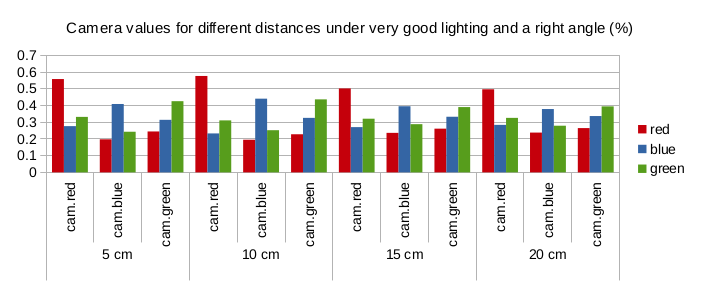
\includegraphics[width=\linewidth]{CamValuesPerc.png}
				\caption{Color measurements in percentage}
			\end{figure}						
			
			\noindent We used this analysis to come up with the following ranges for the 
			colors:
								
			\begin{table}[h!]
				\begin{center}
				\begin{tabular}{c||c|c|c}
					& cam.red & cam.blue & cam.green\\
					\hline
					\hline
					Red & 50\% - 60\% & 15\% - 25\% & 20\% - 30\% \\
					Blue & 20\% - 30\% & 35\% - 45\% & 30\% - 35\% \\
					Green & 30\% - 35\% & 20\% - 30\% & 35\% - 45\% \\ 
				\end{tabular}
				\caption{Color ranges in percentage}
				\label{tab:ColorRanges}
				\end{center}	
			\end{table}
			
			\noindent From the values of Table \ref{tab:ColorRanges} we figured out algorithms 
			to recognize colors. For example, the ratio of red is generally 2 to 4 times bigger 
			than the ratio of blue.	
			\begin{align*}
				2 \cdot cam.blue \leq &cam.red \leq 4 \cdot cam.blue \\
				2 \cdot cam.green \leq &cam.red \leq 3 \cdot cam.green\\
			\end{align*}
			Similarly you can find a calculation for green and blue.
			\begin{align*}
				14 \cdot cam.red \leq 12 \cdot &cam.blue \leq 27 \cdot cam.red \\
				7 \cdot cam.green \leq 7 \cdot &cam.blue \leq 9 \cdot cam.green\\
				\\
				14 \cdot cam.red \leq 12 \cdot &cam.blue \leq 27 \cdot cam.red \\
				7 \cdot cam.green \leq 7 \cdot &cam.blue \leq 9 \cdot cam.green\\
			\end{align*}	
			
		\newpage							
		\subsection{Approach color}
	
\end{document}